% Тут используется класс, установленный на сервере Papeeria. На случай, если
% текст понадобится редактировать где-то в другом месте, рядом лежит файл matmex-diploma-custom.cls
% который в момент своего создания был идентичен классу, установленному на сервере.
% Для того, чтобы им воспользоваться, замените matmex-diploma на matmex-diploma-custom
% Если вы работаете исключительно в Papeeria то мы настоятельно рекомендуем пользоваться
% классом matmex-diploma, поскольку он будет автоматически обновляться по мере внесения корректив
%

% По умолчанию используется шрифт 14 размера. Если нужен 12-й шрифт, уберите опцию [14pt]
\documentclass[14pt]{matmex-diploma}
%\documentclass[14pt]{matmex-diploma-custom}
\usepackage{mathtools}      % матрицы 
\usepackage{amsfonts, amsmath}
\usepackage{multicol,caption,float, subfig} % картинки

\hyphenpenalty=10000    % пенальти на переносы (max)
\sloppy % режим разрешает разрежать строки
\widowpenalty=4000 % пенальти на висячие строки в конце абзаца  
\clubpenalty=4000 % пенальти на висячие строки в начале абзаца

\usepackage{mathtext}
%\usepackage[T2A]{fontenc}
%\usepackage[utf8]{inputenc}
%\usepackage[russian]{babel}


% В предсказании погоды используется множество данных и метеорологических моделей, описывающих физические процессы в атмосфере. С помощью машинного обучения можно исправлять некоторые ошибки этих моделей и улучшать прогнозы погоды. В работе рассматривалось предсказание температуры и предсказание интенсивности осадков. Для улучшения прогноза температуры в данные для обучения модели были добавлены показания с ближайших метеостанций. Они оказались полезны модели для прогнозов на несколько часов вперёд. Для предсказания интенсивности осадков, замеренных метеорологическими радарами, были проведены эксперименты с различной агрегацией данных и способами обучения модели, по итогам удалось достичь значительного улучшения относительно базового решения. Результаты экспериментов оценивались по изменению среднеквадратичной ошибки.
% Weather prediction uses a variety of data and meteorological models describing the physical processes in the atmosphere. With machine learning, some of the errors of these models can be corrected, which improves weather forecasts. This paper considers the prediction of temperature and the prediction of precipitation intensity. To improve the temperature forecast, readings from the nearest meteorological stations were added to the model training data. They have proved useful for the model to predict temperature for the next few hours. To predict the intensity of precipitation measured by weather radars, experiments were carried out with different data aggregation and methods of model training, as a result, a significant improvement has been achieved over the the basic solution. The results of the experiments were evaluated by the change of the root-mean-square error.



\begin{document}
% Год, город, название университета и факультета предопределены,
% но можно и поменять.
% Если англоязычная титульная страница не нужна, то ее можно просто удалить.
\filltitle{ru}{
    faculty = {Математическое обеспечение и администрирование информационных систем},
    chair              = {Информационно-аналитические системы},
    title              = {Методы машинного обучения в задаче предсказания погоды},
    % Здесь указывается тип работы. Возможные значения:
    %   coursework - Курсовая работа
    %   diploma - Диплом специалиста
    %   master - Диплом магистра
    %   bachelor - Диплом бакалавра
    type               = {master},
    position           = {студента},
    group              = 646,
    author             = {Волжина Елена Григорьевна},
    supervisorPosition = {доцент},
    supervisor         = {Михайлова Е.\,Г.},
    %reviewerPosition   = {}
    reviewer           = {Ганьшин А.\,В.},
    chairHeadPosition  = {профессор},
    chairHead          = {Новиков Б.\,А.},
    university         = {Санкт-Петербургский Государственный Университет},
    city               = {Санкт-Петербург},
    year               = {2018}
}
\filltitle{en}{
    faculty = {Software and Administration of Information Systems},
    chair              = {Analytical Information Systems},
    title              = {Machine learning methods in weather prediction problem},
    type               = {master},
    author             = {Elena Volzhina},
    supervisorPosition = {associate professor},
    supervisor         = {Elena Mikhaylova},
    %reviewerPosition   = {assistant},
    reviewer           = {Alexander Ganshin},
    chairHeadPosition  = {professor},
    chairHead          = {Boris Novikov},
    year               = {2018}
}


\maketitle
\tableofcontents


% У введения нет номера главы
% ВВЕДЕНИЕ
\section*{Введение}
С ростом производительности вычислительных систем, объемов накопленных данных об окружающем мире и опыта в их обработке находятся всё новые и новые области для применения анализа данных. Одной из таких областей сегодня является прогнозирование погодных условий и в целом состояния атмосферы. 

Прогнозы погоды полезны как обычным людям для принятия бытовых решений, так и в более серьезных областях: в авиации, судоходстве, а также в сельском хозяйстве. Большую пользу знания о погоде в будущем могут принести и бизнесу, в особенности сезонному, в котором спрос на услуги или возможность проводить работы сильно зависит от погоды.

В Яндексе для прогноза погоды используется технология Метеум, комбинирующая прогнозы от нескольких поставщиков и другие данные с помощью методов машинного обучения, а именно градиентного бустинга над решающими деревьями. Модель, полученная таким образом, улучшает качество прогноза относительно каждого из поставщиков.

В рамках этой работы были рассмотрены две независимые задачи по улучшению прогнозов погодных параметров в Яндекс.Погоде. Во-первых, к используемым температурной моделью данным была добавлена информация о погоде в интересующей нас области в тот момент, когда мы вычисляем свой прогноз. Это может улучшить предсказания для ближайшего будущего, так как оно естественным образом зависит от настоящего. Во-вторых, была разработана новая модель для предсказывания интенсивности осадков.

% численный прогноз погоды https://ru.wikipedia.org/wiki/Численный_прогноз_погоды
% https://ru.wikipedia.org/wiki/Прогноз_погоды 


% ОБЗОР ЛИТЕРАТУРЫ?
\section{Существующие решения}

% про модели, СПИСОК ЛИТЕРАТУРЫ http://method.meteorf.ru/publ/tr/tr359/tolstih.pdf

% на основе lynch2008origins -- история прогнозов
% http://www.mbureau.ru/articles/istoriya-razvitiya-modeley-prognozirovaniya-pogody
% https://habrahabr.ru/post/179687/ -- практически то же, что предыдущее

% от Саши: \cite{васильев2008прогноз} -- познавательный обзор

Наблюдения за погодой и попытки её предсказывать ведутся с тем или иным успехом уже несколько веков. Изначально прогнозы делались на основе опыта наблюдений и примет, но уже в XIX веке с развитием гидродинамики и термодинамики появляются первые математические инструменты для прогнозов. 

К концу XIX века научное сообщество располагало инструментами для исследования поведения газов, законами, описывающими это поведение, а также представлением о крупных системах, обуславливающих состояние атмосферы и, как следствие, погоду в конкретной точке. Были сформулированы идеи о решении системы уравнений с заданными начальными условиями для предсказания погоды в будущем.

В начале XX века Льюис Фрай Ричардсон составил систему уравнений, описывающих процессы, по которым меняется состояние атмосферы. Подставив в качестве начальных условий текущее состояние атмосферы можно было решить систему методом конечных разностей и получить прогноз изменения атмосферного давления\cite{lynch2008origins}. При этом задавать начальные условия требовалось с большой точностью, так как даже небольшая погрешность в них приводила к большим изменениям в результате расчётов. Также значительной проблемой была вычислительная сложность процесса, она делала невозможным сколько-нибудь оперативный прогноз погоды в реальных условиях.

Во второй половине XX века появляются всё новые сведения об атмосферных процессах, уточняющие точность моделирования, а также вычислительные ресурсы и технологии, необходимые для регулярного решения подобных систем в разумных временных рамках. Численное моделирование крупномасштабных явлений в атмосфере значительно улучшилось благодаря информации с искусственных спутников Земли\cite{васильев2008прогноз}.

\subsection{Классические методы}

% https://en.wikipedia.org/wiki/Numerical_weather_prediction
% https://en.wikipedia.org/wiki/Global_Forecast_System
% 

Классический подход к задаче прогноза погоды включает в себя несколько компонентов. В основе всего лежит сбор данных: как долгосрочные наблюдения о температуре, осадках и прочих параметрах в конкретной местности, так и регулярные замеры с помощью разнообразной техники: приборов, установленных на наземных метеостанциях, метеорологических зондов и даже метеорологических спутников. Далее в дело вступают математические модели атмосферы, настроенные с помощью собранных данных. В этих моделях уравнения гидрогазодинамики описывают процессы в атмосфере, которые влияют на интересующие нас величины, а подставив в качестве параметров реальные данные о состоянии атмосферы в данный момент мы можем получить прогноз её состояния через некоторое время.

Модели атмосферы можно разделить на \textit{глобальные}, покрывающие всю планету, и \textit{региональные}, описывающие ограниченную территорию. Первые более универсальны, зато вторые могут давать лучшее качество для своих областей за счет более тонкой настройки и высокого расширения. Сами прогнозы можно разделить на группы по времени, на которое мы смотрим в будущее: \textit{краткосрочные} (до 72 часов), \textit{среднесрочные} (от 72 часов до 10 суток) и \textit{долгосрочные} (более 10 суток).

% дальше инфа от Димы в баре
Построение и обновление математических моделей атмосферы очень трудозатратно и требует проведения большого количества различных экспериментов, поэтому из-за постоянных изменений климата все использующиеся модели являются в большей или меньшей степени устаревшими. Помимо этого, так как физика многих процессов в атмосфере еще недостаточно изучена, у всех моделей есть погрешности в прогнозировании, при этом зачастую эти погрешности имеют постоянную природу: например, одна из моделей может завышать температуру, а другая -- занижать давление в горах. 

Учитывая объемы информации, человеку сложно найти эти шаблоны в ошибках моделей. Но благодаря современным статистическим методам и вычислительным мощностям этот процесс можно автоматизировать. Именно эта идея лежит в основе технологии Метеум, которая используется для прогноза погоды в Яндексе. По накопленным данным о прогнозах разных моделей и фактической погоде в моменты, на которые делались эти прогнозы, можно построить модель, корректирующую прогнозы поставщиков и улучшающую качество итогового прогноза.


\subsection{Машинное обучение, технология Метеум}
% метеум https://habrahabr.ru/company/yandex/blog/271725/
% наукаст https://habrahabr.ru/company/yandex/blog/317626/
% техническая часть наукаста https://habrahabr.ru/company/yandex/blog/328158/
% новая архитектура https://habrahabr.ru/company/yandex/blog/343518/

\textit{Машинным обучением} называют подход к решению задач, заключающийся в анализе большого количества накопленных наблюдений с целью найти в них ранее неизвестные зависимости. Нередко такие зависимости сложно или невозможно (например, в силу недоступности информации о части факторов) описать формально, но благодаря статистическому подходу их можно приблизить с достаточным для практического применения качеством\cite{bishop}.

В задаче предсказания погоды удобно использовать методы \textit{обучения с учителем} -- они применяются, когда на каждое наблюдение, описанное вектором факторов, имеется "правильный ответ". Среди них выделяют методы \textit{классификации}, когда ответом является метка из конечного множества (например, если предсказывается наличие осадков или их тип), и методы \textit{регрессии}, в этом случае ответ -- непрерывная величина (например, температура или количество осадков в миллиметрах).

В качестве примера можно упомянуть The Weather Company, которая для подсчёта прогноза погоды комбинирует информацию из более чем 150 источников данных с помощью машинного обучения\cite{ibm_weather}.

Сервис Яндекс.Погода использует для прогноза погоды технологию Метеум. На основе накопленных данных, которые будут описаны подробнее далее, составляются отдельные модели машинного обучения для интересующих нас параметров: температуры, давления, скорости и направления ветра, а также типа облачности и осадков. Важно уточнить, что температура предсказывается не сама по себе, а как разница между температурой и климатическими данными -- усредненными показаниями за десятки лет для этого времени года. Это позволяет частично избавиться от сезонности в изменениях температуры.

Для обучения в числе прочего используются данные, вычисляемые через классические модели прогнозирования. Сравнивая эти прогнозы с фактическими показаниями, модель находит зависимости целевой переменной от прогнозов разных показателей (например, для осадков кроме, собственно, прогнозов осадков, важными факторами оказываются также прогнозы облачности), а также учится исправлять упомянутые выше погрешности разных моделей.

% В рамках данной работы будет проверена гипотеза о том, что полезной информацией для предсказаний погоды в ближайшем будущем окажется состояние погоды на данный момент. Для этого будут использоваться показания с одной или двух ближайших метеорологических станций.


\begin{figure}
\centering
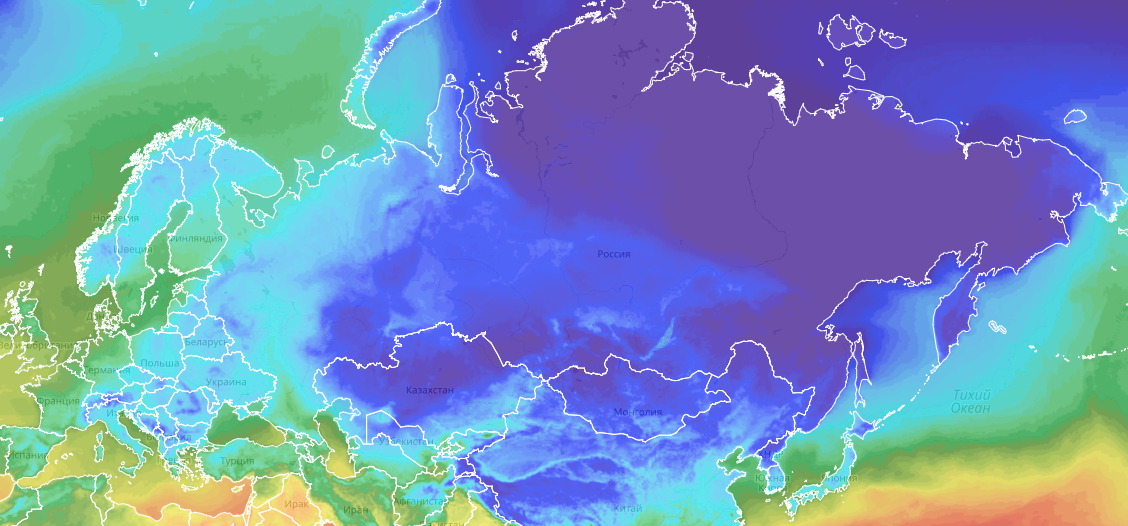
\includegraphics[width=\linewidth]{images/map_coursework.png}
\caption{Карта температуры на Яндекс.Погоде}
\label{fig:map}
\end{figure}



% МЕТОДОЛОГИЯ
\section{Методология}
Прежде чем приступать к экспериментам, следует разобраться с данными, которыми мы располагаем, решить, как мы будем собирать обучающую выборку с известными ответами и готовить её к использованию. Далее нужно выбрать метод для поиска решающей функции, которая бы приближала правильные ответы, находя зависимости в данных. Также необходимо определить метрики, с помощью которых будет приниматься решение, успешным считать эксперимент или нет. После этого можно будет приступать к основным задачам: 

\begin{enumerate}
    \item \textit{задача улучшения прогноза температуры}: требуется добавить к обучающей выборке данные о текущих погодных условиях в месте, для которого рассчитывается прогноз; попробовать обучить на расширенных данных модель для предсказания температуры; оценить по метрикам улучшение;
    \item \textit{задача предсказания интенсивности осадков}: нужно собрать данные об осадках, составить обучающую выборку, определить отправную точку для сравнения качества моделей (\textit{baseline}) и далее проводить эксперименты с целью получить примемлемую по качеству модель.
\end{enumerate}


\subsection{Данные для обучения}
При составлении прогноза мы располагаем множеством данных, полученных от поставщиков или вычисленных самостоятельно. Можно выделить несколько групп этих данных:
\begin{enumerate}
% GFS (США), ECMWF (Англия), JMA (Япония), CMC (Канада), EUMETSAT (Франция), Earth Networks (США) 

    \item \textit{прогнозы погоды}, сделанные при помощи математического моделирования физических процессов в атмосфере; в числе поставщиков следующие глобальные модели: Global Forecast System (GFS \cite{saha2006ncep}), Japan Meteorological Agency (JMA), European Centre for Medium-Range Weather Forecasts (ECMWF \cite{persson2001user}), Canadian Meteorological Centre (CMC). Также на серверах Яндекс.Погоды рассчитывается региональная модель для собственных прогнозов -- Weather Research and Forecasting Model (WRF). У разных моделей могут различаться частота расчётов, координатная сетка, а также набор параметров в прогнозе, это необходимо учитывать при сборе обучающей выборки;

    \item \textit{фактические данные} о погоде, снятые на метеостанциях по всему миру с помощью статических приборов и метеозондов. Используются станции из сети Всемирной метеорологической организации;
    % красивая картинка с вики https://upload.wikimedia.org/wikipedia/commons/5/52/Norman_Doppler_Radar_-_NOAA.jpg
    \item \textit{радарные снимки} осадков и облачности, которые делаются метеорологическими радарами с использованием эффекта Доплера\cite{doviak1993doppler};

    \item \textit{климатические данные}, посчитанные на основе десятков лет наблюдений метеостанций;

    \item \textit{спутниковые снимки}.
\end{enumerate}

Чтобы применять на этих данных какие-либо алгоритмы машинного обучения, нужно очистить их от выбросов и шума, привести всех поставщиков к единой координатной сетке и собрать обучающую выборку. В момент, когда мы делаем прогноз, мы можем использовать полученные ранее прогнозы от поставщиков, статистические данные о климате, а также информацию о погоде в интересующей нас точке в данный момент (или, с учётом задержек в получении данных, в недавнем прошлом).

Нам потребуется множество наблюдений $X = \{x_i = (f^1_{i}, \cdots, f^M_i), i \in \overline{1..N}\}$, элементы которого соответствуют векторам признаков, полезных для предсказывания в текущий момент $gentime$ состояния погоды на момент в будущем $time$. Например, в числе этих признаков будут прогнозы различных погодных параметров: температуры, влажности, скорости и направления ветра, осадков и облачности. Эти прогнозы должны быть сделаны на время, близкое к интересующему нас $time$, при этом при сборе обучающей выборки важно не заглядывать в будущее, то есть время генерации этих прогнозов поставщиками должно быть не позже, чем $gentime$ (а с учётом задержек при передаче данных лучше брать прогнозы, сделанные еще раньше). 

Помимо множества наблюдений $X$ нам понадобится множество целевых значений $y = \{y_i, i \in \overline{1..N}\}$. В контексте первой задачи это разница температуры, которая была получена с метеостанции в момент $time$ (на это время мы делали прогноз), с усредненной за много лет температурой в этот день и в это время: $temperature\_delta = fact\_temperature - climate\_temperature$. Во второй задаче целевыми значениями будут агрегированные данные о миллиметрах выпавших осадков, полученные с метеорадаров.


\subsection{Решающие деревья и градиентный бустинг}

Для проведения экспериментов по прогнозу температуры на основе имеющихся данных был выбран алгоритм \textit{градиентного бустинга над решающими деревьями}. Использовались две реализации этого алгоритма (MatrixNet и CatBoost), разработанные и использующиеся в компании Яндекс.

\textit{Решающее дерево} -- это алгоритм предсказания, описывающийся бинарным деревом, у которого каждой внутренней вершине $v$ поставлен в соответствие некоторый предикат $\beta_v: X \to \{0, 1\}$, а каждому листу соответствует метка с ответом алгоритма\cite{bishop}. После обучения применяется дерево следующим образом: для фиксированного $x \in X$ начинаем с корневой вершины ($v_{root}$). Вычисляем значение $\beta_{v_{root}}(x)$. Если получили $0$, переходим в левого потомка, если $1$ -- в правого. Продолжаем аналогичные вычисления для каждой следующей вершины до тех пор, пока не окажемся в листе, метку которого и возвращаем в качестве ответа.


\textit{Градиентный бустинг} -- алгоритм, с помощью которого по обучающим данным последовательно строится композиция из простых алгоритмов предсказания, причём каждый следующий алгоритм в композиции стремится уменьшить ошибку, которую допускает уже накопленный ансамбль. Такой метод построения называют \textit{жадным}, так как он вместо попытки сразу найти оптимальное решение, идёт к нему итеративно, делая на каждом шаге локально-оптимальный выбор\cite{friedman2001greedy}.

Градиентный бустинг позволяет из простых предсказательных моделей, не приносящих хороших результатов при самостоятельном использовании, получить композицию, хорошо приближающую целевую функцию. При этом модель оказывается устойчивой к переобучению и эффективной в применении (так как элементы композиции можно быстро вычислить параллельно) \cite{FRIEDMAN2002367}.





\subsection{Метрики}
Для ответа на вопрос, улучшают изменения прогноз или ухудшают, необходимо выбрать метрики, с помощью которых в дальнейшем можно будет сравнивать качество разных моделей.

Стандартной метрикой в задаче регрессии (предсказания действительного числа) является \textit{квадратный корень из среднеквадратичной ошибки} (Root Mean Square Error, RMSE). Он показывает, как сильно в среднем прогнозы модели отличаются от фактических данных. Для столбца фактических показаний $y$ и столбца ответов модели $\hat{y}$ значение этой метрики вычисляется следующим образом:
        $$RMSE(y, \hat{y}) = \sqrt{\sum^{n}_{i=1}{(y_i - \hat{y_i})^2}}$$

%Помимо усредненной ошибки нам также хотелось бы понимать, как часто формула ошибается достаточно сильно для того, чтобы вызвать недоумение пользователя сервиса. В качестве порогового значения было выбрано отклонение прогноза от фактической температуры на 5 градусов. Получаем метрику
%        $$Errors_5(y, \hat{y}) = \sum^{n}_{i=1}{[|y_i - \hat{y_i}| > 5]},$$
%    \indent где $[x] = 1\text{, если } x \text{ верно, иначе } 0$.

Чтобы значения метрик объективно отражали качество моделей, нужно считать их на новых для модели примерах. В нашем случае достаточно разделить обучающую выборку на два непересекающихся подмножества ($X_{train}$ и $X_{test}$): наблюдения до определенной даты и после неё, на первом подмножестве обучить модель, а на втором вычислить метрики. Так мы не только будем проверять модель на примерах, которые не встречались ей при обучении, но и не дадим ей подглядывать в будущее (это плохо, так как погоду в последовательные моменты времени нельзя считать независимой).  
%Если бы мы делили $X$ не по дате, а, например, случайным образом, то рисковали бы получить чересчур оптимистичные метрики, ведь модель оценивалась бы по работе на датах, для которых она уже знала gjckt
% Вдобавок таким образом мы получаем оценку положения дел, приближенную к проду

Так как алгоритм градиентного бустинга, как и многие другие, строит модель итеративно, разделение данных на две выборки позволяет также построить \textit{кривые обучения} (learning curves), полезные для анализа способности модели к обобщению. В процессе обучения на каждой итерации для текущей модели вычисляется метрика качества предсказывания на множестве $X_{train}$, на котором она обучается, и на множестве $X_{test}$, которого она ещё не видела. Если в данных есть полезная для предсказывания целевой переменной информация, какое-то количество итераций метрика будет улучшаться на обоих множествах. Но когда модель попадёт в локальный минимум, дальнейшее обучение модели будет приводить к нахождению случайных зависимостей в обучающих данных, что может улучшать метрику на множестве $X_{train}$, но метрика на $X_{test}$ в этом случае будет ухудшаться, так как обобщающая способность модели ухудшится. Такая ситуация называется \textit{переобучением} (overfitting).


\begin{figure}
\centering
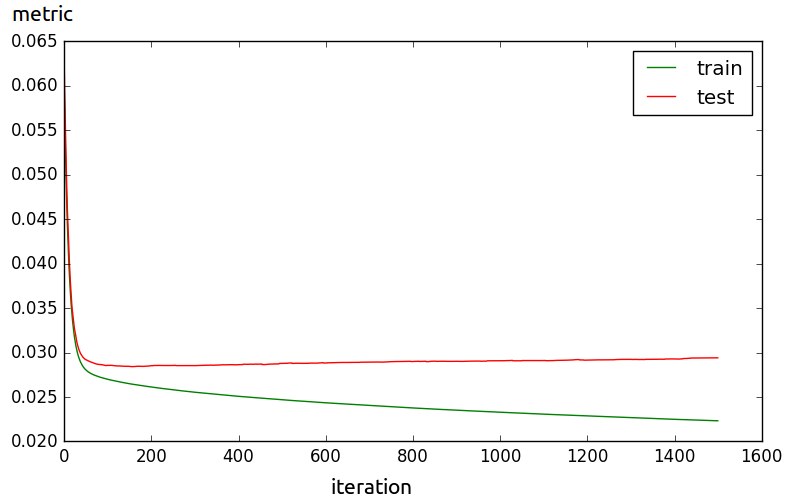
\includegraphics[width=0.9\linewidth]{images/pic6_learning_curves_overfitting.png}
\caption{Типичные кривые обучения для ситуации переобучения}
\label{pic6_learning_curves_overfitting}
\end{figure}




% ЭКСПЕРИМЕНТЫ
\section{Эксперименты: улучшение прогноза температуры}

Для улучшения прогноза погоды в ближайшем будущем было опробовано добавление в обучающую выборку данных о текущей погоде в области, для которой делается прогноз. Обученная модель сравнивалась с использующейся в данный момент в Яндекс.Погоде. Целевой переменной была разница между фактической температурой и средней для этих местности и времени ($temperature\_delta = fact\_temperature - climate\_temperature$).

Данные о текущих погодных условиях могут помочь предсказать погоду в будущем только на небольшой срок. Для экспериментов было выбрано ограничение в 7 часов, и при более дальних прогнозах данные с ближайших станций не использовались.
% Почему 7?

\subsection{Обучающая выборка}
К уже существующей обучающей выборке, собранной из векторов прогнозов поставщиков и других данных в качестве множества наблюдений ($X = \{x_i = (f^1_{i}, \cdots, f^M_i), i \in \overline{1..N}\}$) и реальных $temperature\_delta$ в качестве верных ответов ($y = \{y_i, i \in \overline{1..N}\}$), нужно присоединить данные о фактической погоде в момент генерации прогноза. Для этого было построено следующее соответствие: для каждой станции, с которой поступают фактические данные, вычислены две ближайшие станции в пределах 150 километров. Далее в обучающую выборку для конкретной станции попадают либо данные с этих двух ближайших, либо только с одной из них (а на место второй -- данные с самой станции). %TODO зачеем?

Необходимо при сборе данных для обучения учесть, что в условиях реального применения модели будут задержки в получении данных от поставщиков прогнозов и фактов. Таким образом, если для генерирующегося в момент $gentime$ прогноза мы будем брать фактические данные, снятые на станции в тот же момент $gentime$, мы получим слишком позитивную оценку метрик модели. В реальности задержки имеют порядок десятков минут, и при генерации прогноза на сервисе использоваться будут соответственно устаревшие данные.

% про 30м-3ч30м не хочу писать



\subsection{Удалённость времени прогноза}

Будем называть \textit{горизонтом} прогноза разницу между временем, на которое делается прогноз ($time$), и моментом, когда мы его подсчитываем ($gentime$), в часах.

Для начала был проведен эксперимент с новой обучающей выборкой для всех краткосрочных горизонтов (вплоть до 72-го часа), при этом данные о ближайших станциях были только для первых семи часов. Такое усовершенствование не принесло видимых улучшений, даже на первых семи горизонтах изменения оказались незначительными (Рис.~\ref{pic1_metrics_initial}), что объясняется относительно небольшим числом строк с данными с ближайших станций в обучающей выборке. Эффект от этих данных оказался невысок -- если упорядочить приблизительно 250 признаков каждого наблюдения в обучающей выборке по влиянию на ответ модели, фактор $fact1\_temperature\_delta$ (вычисленный как разница температуры с ближайшей станции и $climate\_temperature$) оказался на 115 месте.
% метрики из https://st.yandex-team.ru/WEATHER-9187#1511946792000, первая картинка

\begin{figure}
\centering
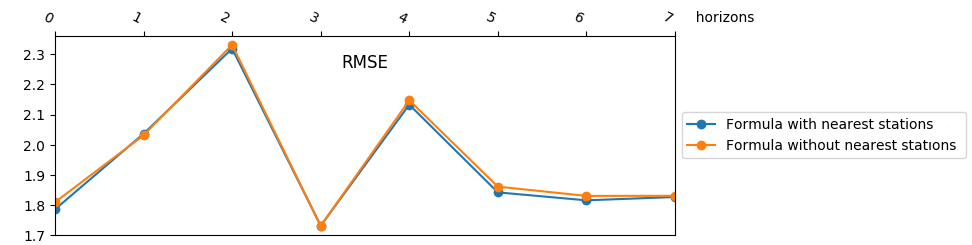
\includegraphics[width=\linewidth]{images/pic1_metrics_initial.png}
\caption{Модели, обученные на всех краткосрочных горизонтах}
\label{pic1_metrics_initial}
\end{figure}


Было решено попробовать обучение отдельной модели только для первых семи часов. Тогда для всех строк в обучающей выборке модель будет знать показания с ближайших станций, благодаря чему эффект от этих данных должен повыситься. Чтобы не увидеть мнимое улучшение относительно базовой модели только за счёт того, что у усовершенствованной модели в обучающей выборке нет удалённых по времени наблюдений с меньшим качеством прогноза у поставщиков, сравнение проводилось с моделью без данных от ближайших станций, но обученной также только на первых 7 часах. Однозначного улучшения по метрикам также не получили, хотя фактор $fact1\_temperature\_delta$ стал вносить значительный вклад в ответ модели -- он оказался на 5 месте по эффекту, наравне с прогнозами температуры от поставщиков.
% метрики из https://st.yandex-team.ru/WEATHER-9187#1512471399000, без картинки
% про fstr Лана написала https://st.yandex-team.ru/WEATHER-9187#1512585426000

Далее были испробованы другие ограничения на число часов, которым ограничивается действие прогноза в будущее, хотелось найти баланс между сокращением применимости модели и улучшением метрик. По результатам экспериментов было выбрано ограничение в 3 часа от момента генерации прогноза. Далее прогнозы полученной модели были нарисованы на карте, чтобы увидеть, как они будут выглядеть для пользователя.
% метрики https://st.yandex-team.ru/WEATHER-9187#1513066306000, странный пик

\begin{figure}
\centering
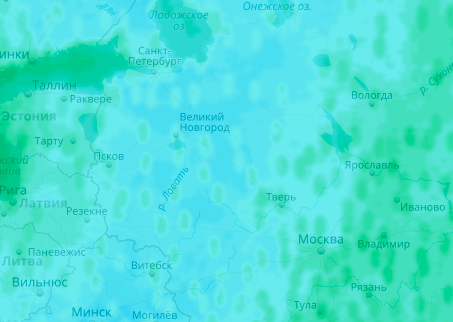
\includegraphics[width=0.6\linewidth]{images/pic2_map.png}
\caption{Пятна вокруг станций}
\label{pic2_map}
\end{figure}

На карте были обнаружены пятна вокруг станций, поставляющих данные (Рис.~\ref{pic2_map}). Они демонстрируют, что раз $temperature\_delta$ с ближайшей станции имеет большой вклад в прогноз модели, то на границе, после которой станция перестаёт считаться ближайшей, и данные от неё для модели пропадают, видны различия в прогнозе.



\subsection{Расстояние до ближайших станций}

Для решения проблемы с пятнами было решено использовать простое сглаживание данных от ближайших станций, чтобы на границе их присутствия не было резкого скачка в значениях. Кроме этого в данные для обучения были добавлены расстояния от точки прогноза до ближайших станций, но по результатам экспериментов они не оказались полезны для модели.

Для сглаживания был взят прогноз самого точного из наших поставщиков, которым подменялись значения с ближайших станций за пределами радиуса их использования ($max\_distance$). Далее для каждого наблюдения для двух ближайших станций были вычислены такие значения: 
\begingroup
\setlength\abovedisplayskip{0pt}
\begin{multline*}
smoothed\_fact\_temperature\_delta := \\\left\{
                \begin{array}{ll}
                  fact \cdot (1 - \frac{dist}{max\_distance}) + forecast \cdot \frac{dist}{max\_distance},\\\indent \text{     if }dist \le max\_distance  \\
                  forecast, \text{ if } dist > max\_distance
                \end{array}
              \right.,
\end{multline*}
\endgroup
\indent где $fact$ -- исходное значение с одной из ближайших станций, $dist$ -- расстояние до неё, а $forecast$ -- прогноз поставщика для точки, где она находится, на момент $time$.


\subsection{Финальное решение}
С описанным выше сглаживанием получили модель, которая показывает лучшие метрики, чем модель, обученная также на первых трёх часах, но без показаний с ближайших станций (Рис.~\ref{pic3_metrics_final}), и при этом не даёт пятен на картах. Сглаженные температуры с двух ближайших станций оказались на 1 и 4 местах по влиянию на ответ модели.
% из графа https://nirvana.yandex-team.ru/flow/47895a5f-63eb-414e-9d80-ab7a45f32724/c601ecaa-a10a-42de-8675-9a5961681231/graph/FlowchartBlockOutput/4c8db20a-7836-46bd-b64c-6a812e8dc488
% чего-то очень большое улучшение

\begin{figure}
\centering
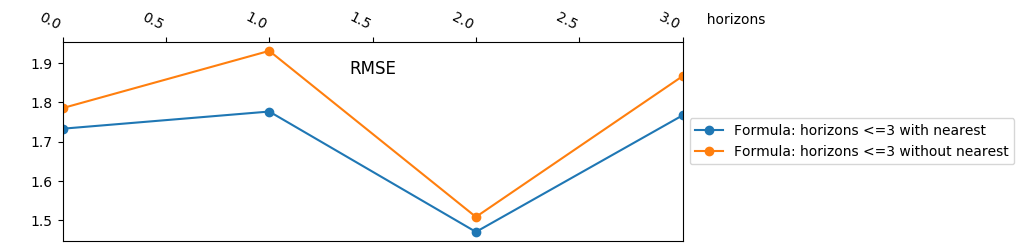
\includegraphics[width=\linewidth]{images/pic3_metrics_final.png}
\caption{Модель с использованием расстояний до ближайших станций}
\label{pic3_metrics_final}
\end{figure}


\section{Эксперименты: прогноз интенсивности осадков}

В этой задаче требовалось создать новую модель, которая бы предсказывала интенсивность осадков, выраженную в миллиметрах за час или иной промежуток времени. Постановка задачи была сделана с учётом бизнес-логики, используемой на сервисе: требовалось предсказывать интенсивность только для случая, когда другая модель уже предсказала сам факт дождя. Таким образом, обучающая выборка должна состоять из наблюдений, для которых целевая переменная строго положительна. В данный момент в Яндекс.Погоде используются прогнозы интенсивности осадков от одного из поставщиков, и именно эти прогнозы будут использоваться в качестве отправной точки для проверки качества новой модели.

\subsection{Обучающая выборка}

В качестве предикторов в обучающем множестве ($X = \{x_i = (f^1_{i}, \cdots, f^M_i), i \in \overline{1..N}\}$) планировалось использовать стандартный набор из признаков, использующихся также и другими моделями в Яндекс.Погоде, с возможностью расширения этого списка теми признаками, которые могут оказать значимый вклад именно для модели, работающей с осадками.

В качестве целевых переменных ($y = \{y_i > 0, i \in \overline{1..N}\}$) можно было бы использовать один из двух источников данных об осадках -- замеры с метеорологических станций или же снимки с метеорологических радаров. Метеорологические станции присылают данные только про локальные осадки, к тому же далеко не для всех станций достоверно известно, за какое время собраны осадки (это может быть и последний час перед замером, и три часа, и больше). В то же время радары отдают данные о некоторой географической окрестности вокруг себя (радиусом порядка 150 километров), и делают это очень часто -- несколько раз в час. Но у них есть и недостатки, обусловленные в основном физикой процесса: у радаров бывают шумовые значения, слепые зоны (не всегда статичные), кроме того некоторые типы облачности могут быть ошибочно приняты за осадки. Тем не менее благодаря большой области покрытия вокруг каждого радара (Рис.~\ref{pic5_radars_map}) и ясной методологии снятия данных для использования в качестве целевых переменных были выбраны данные с радаров.

\begin{figure}
\centering
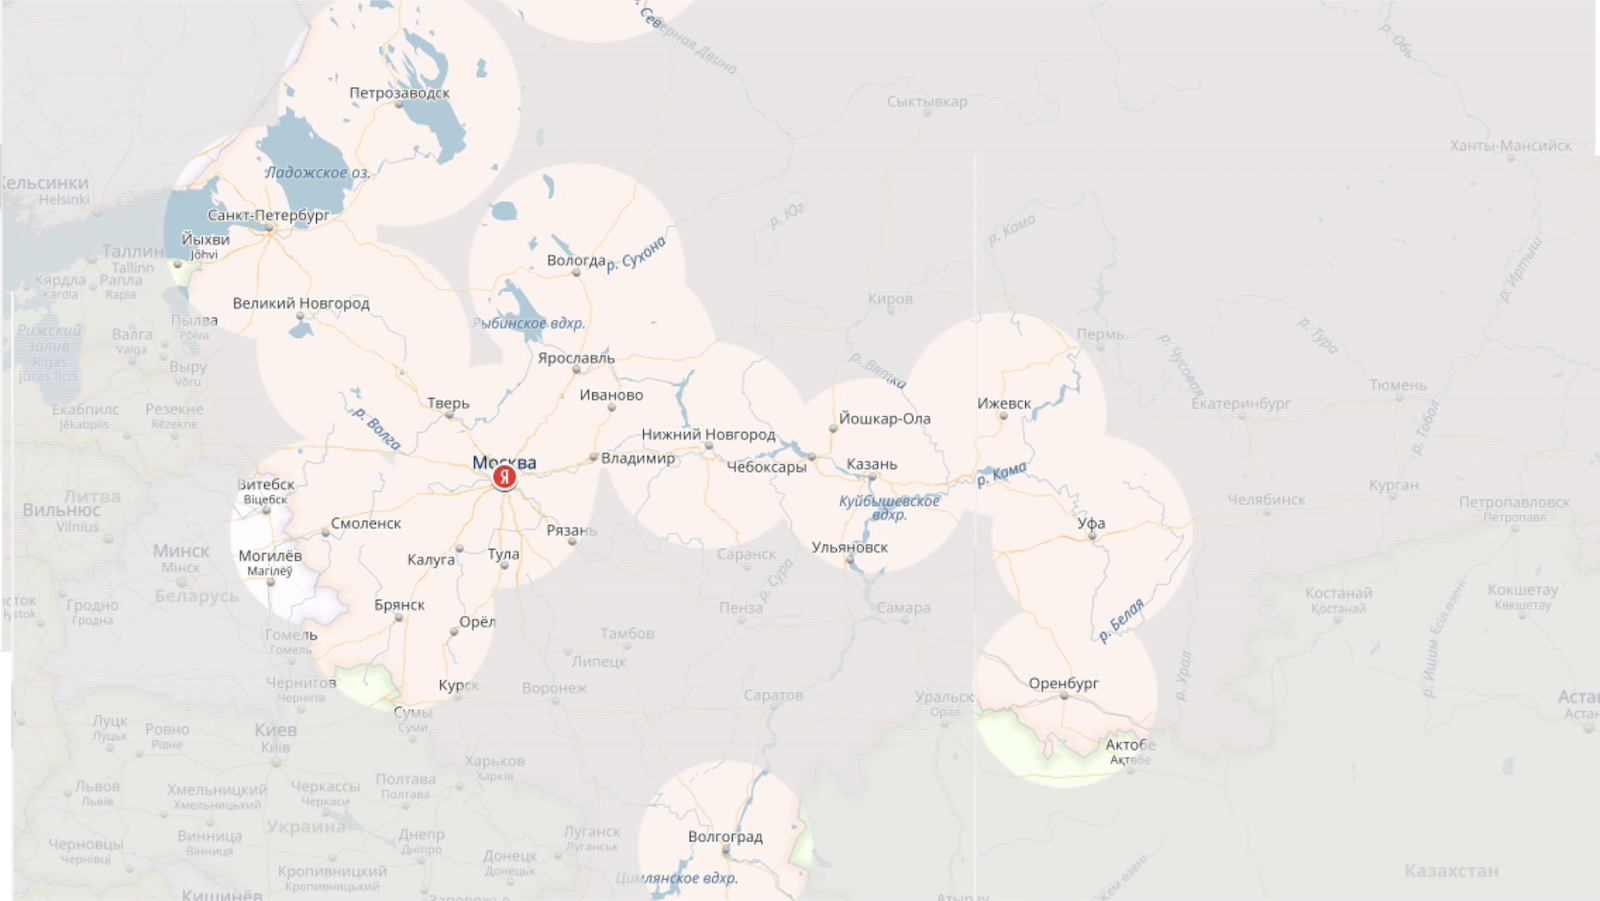
\includegraphics[width=\linewidth]{images/pic5_radars_map.png}
\caption{Область покрытия радаров Росгидромета}
\label{pic5_radars_map}
\end{figure}

% https://habr.com/company/yandex/blog/317626/
% https://habr.com/company/yandex/blog/328158/
% картинка с артефактами: https://hsto.org/web/ff4/b97/b61/ff4b97b612594264a81b30d65fd33011.png

Процесс обработки радарных данных устроен следующим образом:
\begin{itemize}
    \item с заданной периодичностью (в нашем случае раз в 10 минут) с радаров приходят снимки радиусом 150 километров и шагом сетки 2 километра;
    \item все данные для конкретного момента времени склеиваются в один снимок, объединяя места пересечения области видимости радаров по принципу выбора для географической точки максимального значения из всех имеющихся (этап \textit{склейки});
    \item каждый кадр подвергается предобработке (этап \textit{фильтрации});
    \item вокруг точек обучающего множества данные с радаров агрегируются (этап \textit{агрегации});
    \item агрегированные значения присоединяются к обучающему множеству в качестве целевых переменных.
\end{itemize}

В процессе работы над задачей мной были испробованы разные способы фильтрации и агрегации данных, для предшествующих этапов обработки радарных данных были переиспользованы существующие решения.   % перевод: я писала не весь код :)


\subsection{Простой сбор данных}

Для начала работы над задачей были сформулированы следующие требования к данным:
\begin{itemize}
    \item в качестве обучающей выборки использовался стандартный набор данных, составленный из прогнозов поставщиков в точках станций;
    \item данные с радаров суммировались за один час и в окрестности станции с радиусом 3 километра;
    \item для отсечения шумовых значений были выбраны пороги, ограничивающие максимальное количество осадков в миллиметрах как за 10 минут, так и за час;
    \item для агрегации по пространству использовалось три статистики: среднее всех значений в окрестности станции, медиана этих значений, а также среднее, взвешенное расстояниями от станции до точек радарной сетки.
\end{itemize}

На этом этапе из-за вычислительной сложности обработки больших объемов данных обучающая выборка была собрана только по одному месяцу -- октябрю 2017 года.

Чтобы принять во внимание тот факт, что поставщики делают прогнозы не на часовые промежутки, а преимущественно на 3-часовые или же 6-часовые, в обучающую выборку были добавлены для каждого поставщика признаки часа из промежутка предсказания, на который должна сделать прогноз модель.

С таким подходом к формированию обучающей выборки удовлетворительных результатов по метрикам добиться не удалось. Модель проигрывала по RMSE всем поставщикам, в списке наиболее значимых для модели признаков были признаки, не имеющие прямого отношения к осадкам, а кривые обучения показывали быстрое переобучение.


\subsection{Проверка данных}

Нужно было понять, показывает ли модель плохие результаты из-за ошибок при сборе данных, или же сами целевые переменные недостаточно качественные для хорошего предсказывания.

\begin{itemize}
    \item для проверки правильности сбора радарных данных попробовали добавить в обучающее множество данные с радаров за предыдущий час. В реальном применении такие данные использовать невозможно, но так можно было проверить, согласованы ли радарные данные между собой. Модель, обученная на таком наборе данных показала хорошие метрики, а на первом месте по значимости среди признаков оказались данные радаров за предыдущий час, из чего можно сделать вывод, что радары адекватно собраны по географии и времени;
    \item для проверки согласованности прогнозов поставщиков друг с другом попробовали убрать прогноз осадков одного из них из обучающей выборки, а вместо этого использовать его в качестве целевой переменной. Метрики такой модели также оказались удовлетворительными, наибольшую пользу модели принесли прогнозы осадков от других поставщиков, так что данные поставщиков можно считать согласованными;
    \item попробовали также решить вместо регрессионной задачи более простую задачу классификации, превысят ли осадки заданный порог. Проблемы, которые мы видели у регрессии, повторились и у классификации.
\end{itemize}

% перемешанный таргет еще, но не знаю, как это адекватно описать

По результатами этих тестов был сделан вывод, что из-за шумов и артефактов в данных с радаров предсказать их при таких методах фильтрации и агрегации не получится. Было решено изменить требования к данным.


\subsection{Улучшенный сбор данных}

В первую очередь хотелось расширить обучающую выборку, так как при сборе данных за один месяц и только воруг точек метеорологических станций мы получали около 700 тысяч строк в обучающей выборке, которые к тому же были недостаточно разнообразны. Было решено  расширить обучающую выборку с одного месяца до трёх, для этого потребовалось переработать код и улучшить его производительность. Чтобы не ограничиваться при сборе обучающей выборки точками метеорологических станций, стала использоваться сетка с шагом 0.1 градуса, которая покрывала всю область видимости радаров. К узлам этой сетки собирались прогнозы поставщиков и агрегировались радарные данные.

Далее, принимая во внимание, что прогнозы осадков от поставщиков делаются на трех-часовые промежутки, осадки было решено собирать за эти же временные интервалы. Это было сделано из тех соображений, что интенсивность осадков не так плавно меняется со временем, как, например, температура. Из-за этого для практически одинаковых векторов признаков (с прогнозами от поставщиков на трех-часовой интервал) мы могли получить три разных значения целевой переменной.

Кроме этого, чтобы нивелировать воздействие шума от радаров, агрегация стала проводиться не в радиусе 3 километров вокруг точки, для которой делается прогноз, а в радиусе 30 километров.

Наконец, учитывая естественное распределение целевых значений в основном около 0, было решено попробовать три способа установить баланс между маленькими и большими осадками. Во-первых, это логарифмирование целевой переменной, а также расширение обучающей выборки логарифмированными прогнозами осадков от поставщиков. Во-вторых, можно разделить обучающую выборку на две: строки со значениями целевой переменной из интервала $(0, 1]$ и остальные строки, и обучить две отдельные модели. В-третьих, располагая после улучшений в сборе данных большими объемами разнообразных целевых значений, не составит труда собрать обучающую выборку с нужным балансом больших, средних и маленьких осадков. Также можно попробовать увеличить вес при обучении модели для тех строк сбалансированной выборки, в которых целевая переменная больше некоторого порога.

В процессе экспериментов выяснилось также, что на собранных данных реализация алгоритма градиентного бустинга CatBoost склонен к переобучению значительно меньше, чем предшествующая ему реализация, использовавшаяся до сих пор -- MatrixNet. Дальнейшие эксперименты проводились с использованием CatBoost.


\subsection{Текущие результаты}

В таблицах \ref{table_simple_pool} и \ref{table_balanced_pool} можно увидеть сравнение восьми моделей, описанных выше, с прогнозами поставщика, используемого сейчас в Яндекс.Погоде для предсказания интенсивности осадков. Сравнение проводилось на тестовой части выборки, которую модели не видели при обучении -- туда отнесены 20 дней октября 2017 года. Как можно заметить, каждая из представленных моделей показывает качество прогноза лучше, чем у используемых сейчас прогнозов метеорологической модели. Для лучшего понимания применимости этих моделей в реальных условиях потребуется более детально рассмотреть отдельные классы осадков (слабый дождь, сильный дождь, ливень) и посчитать качество прогноза на них. Например, модели, обученные на промежутке $(0, 1]$, скорее всего будут очень плохо предсказывать сильные дожди, в то время как модели, обученные на сбалансированном наборе данных, будут проигрывать в точности предсказания слабых дождей.


% metrics @ test: https://paste.yandex-team.ru/470225
% TODO: вопрос про неоднородность данных в трейне и тесте или другом тесте

\begin{table}[H]
  \centering
  \begin{tabular}{ l | r | r }
     & model RMSE & provider RMSE \\ 
     \hline
    simple regression, any target &  0.5386  &  0.8431 \\ 
    log precipitation, any target &  0.5482  &  0.8431 \\ 
    simple regression @ $(0, 1]$  &  0.1890  &  0.7165 \\ 
    log precipitation @ $(0, 1]$  &  0.1898  &  0.7165 \\ 
  \end{tabular}
  \caption{RMSE моделей, обученных на обычной обучающей выборке}
  \label{table_simple_pool}
\end{table}

\begin{table}[H]
  \centering
  \begin{tabular}{ l | r | r }
     & model RMSE & provider RMSE \\ 
    simple regression             &  1.6231  &  1.8527 \\ 
    log precipitation             &  1.6977  &  1.8527 \\ 
    simple regression + weights   &  1.6695  &  1.8527 \\ 
    log precipitation + weights   &  1.7330  &  1.8527 \\ 
  \end{tabular}
  \caption{RMSE моделей, обученных на сбалансированной обучающей выборке}
  \label{table_balanced_pool}
\end{table}






% У заключения нет номера главы
\section*{Заключение}
В рамках данной работы была проверена гипотеза о том, что данные с ближайших метеорологических станций будут полезны для предсказаний температуры. Также были построены и исследованы несколько моделей для предсказания интенсивности осадков.

\subsubsection*{Улучшение прогноза температуры}

При работе над первой задачей было показано, что данные с ближайших станций могут помочь улучшить прогноз температуры. По итогам экспериментов оказалось, что польза от этих данных сохраняется в течение нескольких часов. Использовать показания со станций нужно с некоторым сглаживанием, чтобы не получить ярко выраженных окрестностей вокруг станций. 

Полученная в результате экспериментов модель показала значительный выигрыш по метрике средне-квадратичного отклонения относительно модели, использовавшейся прежде. %Описанная реализация модели в данный момент уже используется в Яндекс.Погоде.

Выводы, сделанные при работе над прогнозом температуры, можно попробовать применить и для прогноза других погодных параметров, для которых показания с ближайших станций также могут дать полезную для моделей информацию.



%В качестве возможных направлений развития этой задачи перечислю следующие:
%\begin{itemize}
%    \item использовать ближайшие станции для предсказания не только $temperature\_delta$, но и других показателей;
%    \item использовать кросс-валидацию, чтобы уменьшить влияние конкретного разбиения на обучающую и тестовую выборки и более объективно оценивать изменения;
%    \item поэкспериментировать с параметрами градиентного бустинга, по первым шагам в этом направлении похоже, что возможны значительные улучшения (Рис.~\ref{pic4_params});
%    \item попробовать другие способы сглаживания показаний со станций по мере удаления точки прогноза от них. 
%\end{itemize}


% картинка из https://nirvana.yandex-team.ru/flow/47895a5f-63eb-414e-9d80-ab7a45f32724/79a0c479-4853-4e40-a8a1-3dcba92479c4/graph
%\begin{figure}
%\centering
%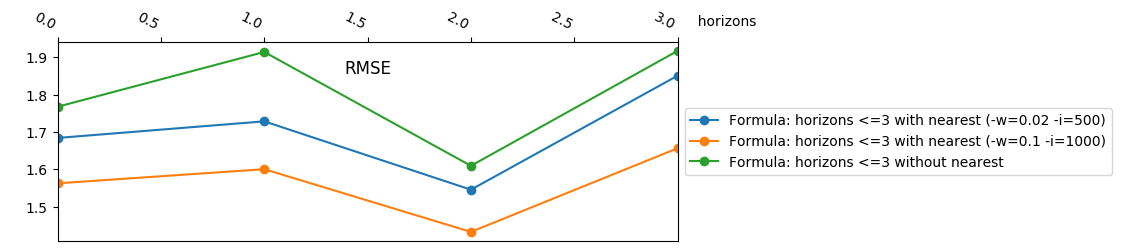
\includegraphics[width=\linewidth]{images/pic4_params.png}
%\caption{Эксперимент с параметрами алгоритма MatrixNet}
%\label{pic4_params}
%\end{figure}


\subsubsection*{Прогноз интенсивности осадков}

При построении модели для прогноза осадков был пройден весь путь от выбора способа формирования обучающей выборки и целевых переменных до финальной оценки полученных моделей и сравнения с базовым решением, которое используется в Яндекс.Погоде сейчас.

При сборе данных было испробовано несколько методов агрегации снимков, полученных с метеорологических радаров. Начальный способ не позволил построить модель с хорошим качеством, но его удалось усовершенствовать и собрать обучающую выборку, из которой модели удалось извлечь необходимые зависимости в данных. Также были исследованы разные способы обучения моделей на собранной выборке. 

В результате по нескольким полученным моделям проведен сравнительный анализ качества прогнозов моделей и используемого сейчас решения. Каждая из моделей показала улучшение относительно базового решения.



%Для завершения данного этапа построения модели требуется выбрать из полученных моделей одну на основе более детальных метрик о качестве прогнозов нескольких классов осадков.

%Далее возможные шаги по улучшению прогноза таковы:
%\begin{itemize}
%    \item расширение обучающей выборки ещё несколькими месяцами, желательно насыщенных осадками (к примеру, можно взять ещё два месяца лета 2017);
%    \item разработка моделей для иных типов осадков;
%    \item анализ данных от радаров с целью отсечь шумы и артефакты;
%    \item добавление признаков, которые в моделях для других погодных параметров не приносили пользы, но имеют ценность для прогноза осадков;
%    \item анализ данных с метеорологических станций, которые дают достоверные данные об осадках -- эти данные могут помочь дополнительно оценивать прогнозы моделей без долгой обработки радарных данных;
%\end{itemize}



\setmonofont[Mapping=tex-text]{CMU Typewriter Text}
\bibliographystyle{ugost2008ls}
\bibliography{diploma.bib} 
\end{document}
